\documentclass[11pt]{article}
\usepackage[T1]{fontenc}
\usepackage[utf8]{inputenc}
\usepackage[letterpaper]{geometry}

\usepackage{graphicx}
\usepackage{mathpazo}

\usepackage{amsmath}
\usepackage{amsfonts}
\usepackage{bm}
\usepackage{siunitx}
\usepackage{cancel}
\usepackage{float}
\usepackage{empheq}
\usepackage[most]{tcolorbox}
\usepackage{subcaption}

% Sexy yellow highlighted boxed equations!
\newtcbox{\mymath}[1][]{%
  nobeforeafter, math upper, tcbox raise base,
  enhanced, colframe=black!30!black,
  colback=yellow!30, boxrule=1pt,
  #1}

% Hyperlinks with decent looking default colors.
\usepackage{hyperref}
\usepackage{xcolor}
\hypersetup{
  colorlinks,
  linkcolor={red!50!black},
  citecolor={blue!50!black},
  urlcolor={blue!80!black}
}

% For those sexy spaced low small caps from classic-thesis!
\usepackage{microtype}
\usepackage{textcase}
\DeclareRobustCommand{\spacedlowsmallcaps}[1]{%
  \textls[80]{\scshape\MakeTextLowercase{#1}}%
}

% Replaced mathpazo \sum symbol with computer modern's.
\DeclareSymbolFont{cmlargesymbols}{OMX}{cmex}{m}{n}
\let\sumop\relax
\DeclareMathSymbol{\sumop}{\mathop}{cmlargesymbols}{"50}

% Force indent command.
\newcommand{\forceindent}{\leavevmode{\parindent=1em\indent}}

% Math shortcuts.
\newcommand\p[2]{\frac{\partial #1}{\partial #2}}
\newcommand\G[6]{\p{g_{#1 #2}}{#5}\p{g_{#3 #4}}{#6}}

% fancyhdr header and footer.
\usepackage{fancyhdr}
\pagestyle{fancy} 
\fancyhead{}
\rhead{Ali Ramadhan}
\lhead{6.339 Project 3---Finite Element Methods}
\cfoot{\thepage}

\title{\spacedlowsmallcaps{6.339: Numerical Methods for Partial Differential Equations}\\ \spacedlowsmallcaps{Project three: Finite Element Methods}}
\author{Ali Ramadhan$^\text{†}$ (\href{mailto:alir@mit.edu}{\texttt{alir@mit.edu}})}
\date{\textit{$^\text{†}$Department of Earth, Atmospheric, and Planetary Sciences}}

\renewcommand\thesubsection{\thesection(\alph{subsection})}

\begin{document}
\maketitle

In this project, we will utilize finite element methods to study the deflection or bending of beams by solving the linear elasticity equation. It assumes that the strains and deformations are small, thus yielding a linear relationship between the stress and strain components.\footnotemark~In its most general form, it can be expressed as a balance of linear momentum using Newton's second law
\begin{equation*} \label{eq:linElasGen}
  \bm{\nabla\cdot\sigma + f} = \rho\ddot{\bm{u}}
\end{equation*}
where $\bm{\sigma}$ is the \emph{Cauchy-stress tensor}, $\bm{f}$ is the body force per unit volume, $\rho$ is the mass density, and $\ddot{\bm{u}}$ is the second time derivative of the deformation vector $\bm{u}$. The Cauchy-stress tensor is a second-order or rank-2 tensor. Its diagonal components $\sigma_{kk}$ represent the normal stresses while the off-diagonal components $\sigma_{ij} \; (i \ne j)$  represent the shear stresses at a point. The $\sigma_{ij}$ component corresponds to the stress acting on a plane normal to the $x_i$-axis in the direction of the $x_j$-axis.

\footnotetext{The more general theory of nonlinear elasticity, or finite strain theory, can be used to model arbitrarily large strains and rotations as well as nonlinear stress-strain relations involving effects such as buckling, yielding, and plasticity.}

In two dimensions the linear elasticity equation can be expanded and written as
\begin{equation} \label{eq:linElas}
  \p{\bm{\sigma}_x(\bm{u})}{x} + \p{\bm{\sigma}_y(\bm{u})}{y} + \bm{f} = 0
\end{equation}
where $\bm{u} = (u_x, u_y)$, $\bm{\sigma}_x = (\sigma_{xx}, \sigma_{xy})$ and $\bm{\sigma}_y = (\sigma_{yx}, \sigma_{yy})$ are the stress vector fields, and $\bm{f} = (f_x, f_y)$, all of which are multivariate functions of $x$ and $y$. We are interested in studying the bending of a beam under equilibrium, that is when all the forces on the beam sum to zero and thus the displacement is time-independent. In this elastostatic regime $\ddot{\bm{u}} = 0$ and thus we are left with a set of time-independent partial differential equations.

In order to solve for the displacement field $\bm{u}(x,y)$, we require more information to relate the components of the stress tensor $\sigma_{ij}(x,y)$ to the displacements $u_x(x,y)$ and $u_y(x,y)$. This information comes in the form of a set of strain-displacement relations and a constitutive relation. In their most general form, the strain-displacement relation can be expressed as
\begin{equation*}
  \bm{\varepsilon} =\frac{1}{2} \left[ \bm{\nabla u} + (\bm{\nabla u})^T \right]
\end{equation*}
while the constitutive relation is \emph{Hooke's Law}, $\bm{\sigma} = \bm{C : \varepsilon}$ where $\bm{\varepsilon}$ is the \emph{infinitesimal strain tensor} and $\bm{C}$ is the rank-4 \emph{stiffness tensor}. $\bm{M}^T$ represents the transpose of the matrix $\bm{M}$ and $\bm{A:B} = A_{ij}B_{ij}$ is the inner product for rank-2 tensors where summation over repeated indices is implied as per the \emph{Einstein summation convention}, or rather a small borrowing from the notation of Ricci calculus if you prefer.

In our case we are given the strain-displacement relations and the constitutive relation together, directly relating the stresses to the displacements by the matrix equation
\begin{equation}
\begin{pmatrix}
  \sigma_{xx} \\
  \sigma_{xy} \\
  \sigma_{yx} \\
  \sigma_{yy}
\end{pmatrix}
=
\frac{E}{1-\nu^2}
\begin{pmatrix}
  1 & 0 & 0 & \nu \\
  0 & \frac{1-\nu}{2} & \frac{1-\nu}{2} & 0 \\
  0 & \frac{1-\nu}{2} & \frac{1-\nu}{2} & 0 \\
  \nu & 0 & 0 & 1
\end{pmatrix}
\begin{pmatrix}
\p{u_x}{x} \\
\p{u_x}{y} \\
\p{u_y}{x} \\
\p{u_y}{y}
\end{pmatrix}
\end{equation}
where $E$ is the \emph{Young's modulus} and $\nu$ the \emph{Poisson ratio} of the material. Expanding out the matrix equation and noticing that $\sigma_{xy} = \sigma_{yx}$ as expected due to the symmetric nature of the stress tensor, we obtain relations between $\bm{\sigma}$ and the spatial derivatives of $\bm{u}$
\begin{equation} \label{eq:sigmaComp}
\begin{gathered}
  \sigma_{xx} = \frac{E}{1-\nu^2} \left( \p{u_x}{x} + \nu\p{u_y}{y} \right) \\
  \sigma_{yy} = \frac{E}{1-\nu^2} \left( \nu\p{u_x}{x} + \p{u_y}{y} \right) \\
  \sigma_{xy} = \sigma_{yx} = \frac{E}{1-\nu^2} \left( \frac{1-\nu}{2} \right) \left(\p{u_x}{y} + \p{u_y}{x} \right)
\end{gathered}
\end{equation}

\section{Mathematical foundations}
Before we can develop a solution method or numerical scheme utilizing the finite element method, we will first express the partial differential equations in a \emph{weak formulation} admitting \emph{weak solutions} that may not be sufficiently differentiable to satisfy the strong formulation yet satisfy the weak formulation and represent physically realizable solutions. For the linear elasticity equation in particular, it so happens that the weak and strong formulations are actually equivalent \cite{Tchonkova011}.

\subsection{Derivation of the weak form of the linear elasticity equation}
Expanding the linear elasticity equation \eqref{eq:linElas} yields two partial differential equations
\begin{subequations}
\begin{gather}
  \p{\sigma_{xx}}{x} + \p{\sigma_{xy}}{y} + f_x = 0 \\
  \p{\sigma_{yx}}{x} + \p{\sigma_{yy}}{y} + f_y = 0
\end{gather}
\end{subequations}
which we can write more compactly
\begin{equation*} \label{eq:linElasij}
  \p{\sigma_{jx}}{x} + \p{\sigma_{jy}}{y} + f_j = 0, \quad j=1,2
\end{equation*}
where $j=1,2$ or $j=x,y$ indexes the two equations so that the subscript 1 corresponds to the $x$ coordinate while $2$ corresponds to the $y$ coordinate.

We will now multiply \eqref{eq:linElasij} by a \emph{test function} $\bm{g} = (g_x,g_y)$ and integrate over the domain of the problem $\Omega$ to obtain
\begin{equation*}
  \iint_\Omega g_j(x,y) \left( \p{\sigma_{jx}}{x} + \p{\sigma_{jy}}{y} + f_j \right) \, dA = 0
\end{equation*}
We note that the components of $\bm{g}$ belong to a \emph{Sobolev space} $\mathcal{X}$ so that $\bm{g} \in \mathcal{X}\times\mathcal{X}$. In our particular case we will take $\mathcal{X} = H^1_\Omega$, the Hilbert space of once-differentiable square integrable functions, that is
\begin{equation*}
  H^1_\Omega = \left\{ f(x) : \int_\Omega f^2(x) \, dx < \infty, \quad \int_\Omega \left\lVert \nabla\cdot f \right\rVert < \infty \right\}
\end{equation*}

Then expanding we obtain
\begin{equation*}
\iint_\Omega g_j  \left( \p{\sigma_{jx}}{x} + \p{\sigma_{jy}}{y} \right) \, dA + \iint_\Omega g_j f_j \, dA = 0
\end{equation*}
where we notice that the first integral's integrand is a divergence of $\bm{\sigma}_j$ and so we can write
\begin{equation} \label{eq:ph1}
\iint_\Omega g_j \left( \bm{\nabla \cdot \sigma}_j \right) \, dA + \iint_\Omega g_j f_j \, dA = 0
\end{equation}
Now we can make use of \emph{Green's theorem} to rewrite the first term as
\begin{equation*}
  \iint_\Omega g_j \left( \bm{\nabla \cdot \sigma}_j \right) \, dA
  = \int_{\partial\Omega} g_j  \left( \bm{\sigma_j \cdot \hat{n}} \right) \, d\ell
  - \iint_\Omega \nabla g_j \cdot \bm{\sigma_j} \, dA
\end{equation*}
where $\partial\Omega$ denotes the boundary of the domain of integration $\Omega$, $\bm{\hat{n}}$ denotes the unit normal vector pointing to the outside of $\Omega$ along the boundary $\partial\Omega$, and $d\ell$ denotes a line element along $\partial\Omega$ thus making the middle term a line integral. Rearranging the equation we can write \eqref{eq:ph1} as
\begin{equation}
  \int_{\partial\Omega} g_j  \left( \bm{\sigma}_j \cdot \bm{\hat{n}} \right) \, d\ell
  - \iint_\Omega \nabla g_j \cdot \bm{\sigma_j} \, dA
  + \iint_\Omega g_j f_j \, dA = 0
\end{equation}

Adding the two equations for $j=1,2$ together we obtain
\begin{equation} \label{eq:withLI}
    \int_{\partial\Omega} \left( \bm{\sigma}_x n_x + \bm{\sigma}_y n_y \right) \, d\ell
  - \iint_\Omega \left( \nabla g_x \cdot \bm{\sigma_x} + \nabla g_y \cdot \bm{\sigma_y} \right) \, dA
  + \iint_\Omega \left( g_x f_x + g_y f_y \right) \, dA= 0
\end{equation}
as both equations equalled zero independently. We notice that the first term goes to zero because of the free boundary condition  $\bm{\sigma}_x n_x + \bm{\sigma}_y n_y = 0$ we are imposing. Expanding the gradient terms and the dot products then further rearranging we get
\begin{equation}
  \iint_\Omega \left( \p{g_x}{x}\sigma_{xx} + \p{g_x}{y}\sigma_{xy} + \p{g_y}{x}\sigma_{yx} + \p{g_y}{y}\sigma_{yy} \right) \, dA = \iint_\Omega \left( g_x f_x + g_y f_y \right) \, dA
\end{equation}
into which we can substitute the relations for $\sigma_{ij}$ from \eqref{eq:sigmaComp} yielding
\begin{multline}
  \iint_\Omega \frac{E}{1-\nu^2} \left\{
    \p{g_x}{x} \left( \p{u_x}{x} + \nu\p{u_y}{y} \right)
    + \frac{1-\nu}{2} \left( \p{g_x}{y} + \p{g_y}{x} \right)
      \left( \p{u_x}{y} + \p{u_y}{x} \right) \right. \\ \left.
    + \p{g_y}{y} \left(\nu\p{u_x}{x} + \p{u_y}{y} \right)
  \right\} \, dA
  - \iint_\Omega \left( g_x f_x + g_y f_y \right) \, dA
  = 0
\end{multline}

Tgys we have our weak formulation for the linear elasticity equation for our particular case which takes on the form
\begin{equation} \label{eq:weakForm}
  a(\bm{u,g}) + \ell(\bm{g}) = 0 \quad \forall \bm{u,g} \in H^1_\Omega \times H^1_\Omega
\end{equation}
where $a(\bm{u,g})$ is a bilinear form and
\begin{multline} \label{eq:aug}
  a(\bm{u,g}) =
  \iint_\Omega \frac{E}{1-\nu^2} \left\{
    \p{g_x}{x} \left( \p{u_x}{x} + \nu\p{u_y}{y} \right)
    + \frac{1-\nu}{2} \left( \p{g_x}{y} + \p{g_y}{x} \right)
      \left( \p{u_x}{y} + \p{u_y}{x} \right) \right. \\ \left.
    + \p{g_y}{y} \left(\nu\p{u_x}{x} + \p{u_y}{y} \right)
  \right\} \, dA
\end{multline}
and
\begin{equation} \label{eq:lg}
  \ell(\bm{g}) = - \iint_\Omega \left( g_x f_x + g_y f_y \right) \, dA
\end{equation}

\subsubsection*{Proof for the symmetric and positive-definiteness of the weak form}
A bilinear form $a(u,v)$ that is \emph{symmetric} obeys the property $a(u,v) = a(v,u)$ for all $u,v$. To see that our blinear form $a(\bm{u,g})$ from \eqref{eq:aug} is symmetric, we can explicitly compute
\begin{multline}
  a(\bm{g,u}) =
  \iint_\Omega \frac{E}{1-\nu^2} \left\{
    \p{u_x}{x} \left( \p{g_x}{x} + \nu\p{g_y}{y} \right)
      + \frac{1-\nu}{2} \left( \p{u_x}{y} + \p{u_y}{x} \right)
      \left( \p{g_x}{y} + \p{g_y}{x} \right) \right. \\ \left.
    + \p{u_y}{y} \left(\nu\p{g_x}{x} + \p{g_y}{y} \right)
  \right\} \, dA \\
  = \iint_\Omega \frac{E}{1-\nu^2} \left\{
  \p{u_x}{x} \p{g_x}{x} + \nu \p{u_x}{x} \p{g_y}{y}
  + \frac{1-\nu}{2} \left( \p{g_x}{y} + \p{g_y}{x} \right)
  \left( \p{u_x}{y} + \p{u_y}{x} \right) \right. \\ \left.
  + \nu\p{u_y}{y}\p{g_x}{x} + \p{u_y}{y}\p{g_y}{y}
  \right\} \, dA \\
  =   \iint_\Omega \frac{E}{1-\nu^2} \left\{
  \p{g_x}{x} \left( \p{u_x}{x} + \nu\p{u_y}{y} \right)
  + \frac{1-\nu}{2} \left( \p{g_x}{y} + \p{g_y}{x} \right)
  \left( \p{u_x}{y} + \p{u_y}{x} \right) \right. \\ \left.
  + \p{g_y}{y} \left(\nu\p{u_x}{x} + \p{u_y}{y} \right)
  \right\} \, dA \\
  \hspace{3.5em} = a(\bm{u,g}) \hfill
\end{multline}

A bilinear form that is \emph{positive semidefinite} obeys the property $a(u,v) \ge 0$ for all $u,v$. Additionally, symmetric bilinear forms that satisfy $a(u,u) \ge 0$ for all nonzero $u$ satisfy the positive semidefinite property as well \cite{mathworld}. We thus see that
\begin{multline}
  a(\bm{u,u}) =
  \iint_\Omega \frac{E}{1-\nu^2} \left\{
    \p{u_x}{x} \left( \p{u_x}{x} + \nu\p{u_y}{y} \right)
      + \frac{1-\nu}{2} \left( \p{u_x}{y} + \p{u_y}{x} \right)
      \left( \p{u_x}{y} + \p{u_y}{x} \right) \right. \\ \left.
    + \p{u_y}{y} \left(\nu\p{u_x}{x} + \p{u_y}{y} \right)
  \right\} \, dA \\
  = \iint_\Omega \frac{E}{1-\nu^2} \left\{
  \p{u_x}{x} \p{u_x}{x} + \nu\p{u_x}{x}\p{u_y}{y}
  + \frac{1-\nu}{2} \left( \p{u_x}{y} + \p{u_y}{x} \right)^2 
  + \nu\p{u_y}{y}\p{u_x}{x} + \p{u_y}{y} \p{u_y}{y}
  \right\} \, dA \\
  = \iint_\Omega \frac{E}{1-\nu^2} \left\{
  \left( \p{u_x}{x} \right)^2 + 2\nu\p{u_y}{y}\p{u_x}{x} + \left( \p{u_y}{y} \right)^2
  + \frac{1-\nu}{2} \left( \p{u_x}{y} + \p{u_y}{x} \right)^2
  \right\} \, dA
\end{multline}
where we have that
\begin{equation*}
	\left( \p{u_x}{x} \right)^2 + 2\nu\p{u_y}{y}\p{u_x}{x} + \left( \p{u_y}{y} \right)^2
	\ge \nu \left( \p{u_x}{x} \right)^2 + 2\nu\p{u_y}{y}\p{u_x}{x} + \nu \left( \p{u_y}{y} \right)^2
	= \nu \left(  \p{u_x}{x} + \p{u_y}{y} \right)^2
\end{equation*}
as Poisson's ratio $\nu$ must obey $-1 < \nu < 0.5$ for the isotropic materials under consideration for this project \cite{Mott09}. Therefore
\begin{equation*}
	a(\bm{u,u})
	\ge \iint_\Omega \frac{E}{1-\nu^2} \left\{
		\nu \left(  \p{u_x}{x} + \p{u_y}{y} \right)^2
		+ \frac{1-\nu}{2} \left( \p{u_x}{y} + \p{u_y}{x} \right)^2
	\right\} \, dA
	\ge 0
\end{equation*}
assuming that $\nu > 0$ as the integrand will always be positive. Indeed, $0.2 < \nu < 0.5$ for the vast majority of engineering materials \cite{Mott09}, and $\nu = 0.31$ in our case, so the weak form is certainly positive semidefinite, $a(\bm{u,u}) \ge 0$, for the purposes of this project.

\subsection{Discretization of the weak form}
We will discretize the weak form over the square domain $\Omega = [-1,1]\times[-1,1]$. We'll begin by expressing our variables of interest $\bm{u}$ and test functions $\bm{g}$ in terms of a set of bilinear basis functions
\begin{equation}
\begin{gathered}
g_{--}(x,y) = \frac{(1+x)(1+y)}{4}, \quad g_{-+}(x,y) = \frac{(1+x)(1-y)}{4}\\
g_{+-}(x,y) = \frac{(1-x)(1+y)}{4}, \quad g_{++}(x,y) = \frac{(1-x)(1-y)}{4}
\end{gathered}
\end{equation}
As we are expressing both $\bm{u}$ and $\bm{g}$ in terms of the same basis functions, we are in effect employing a \emph{Galerkin method}, which is simplified when dealing with a symmetric and positive-definite bilinear weak form $a(\bm{u,g})$.

This allows us to express, for example, $u_x(x,y)$ as a linear combination of the basis functions
\begin{equation}
  u_x(x,y) = a_{ij}g_{ij}(x,y) \equiv \sumop_{i,j \in \{-,+\}} a_{ij}g_{ij}(x,y)
\end{equation}
where summation over the repeated indices $i,j$ is now implied. Doing this for each component of $\bm{u}$ and $\bm{g}$ we can write
\begin{equation}
\begin{gathered}
  u_x(x,y) = a_{ij}g_{ij}(x,y), \quad u_y(x,y) = b_{ij}g_{ij}(x,y) \\
  g_x(x,y) = c_{ij}g_{ij}(x,y), \quad g_y(x,y) = d_{ij}g_{ij}(x,y)
\end{gathered}
\end{equation}
where the $\bm{u}$ components get the $a_{ij}$ and $b_{ij}$ coefficients while the $\bm{g}$ components get the $c_{ij}$ and $d_{ij}$ coefficients. Plugging these into the weak form, we get
\begin{multline}
  a(\bm{u},\bm{g}) = \frac{E}{1-\nu^2} \iint_\Omega \left\{
    c_{ij}\p{g_{ij}}{x} \left(
      a_{kl}\p{g_{kl}}{x}
      + \nu b_{kl}\p{g_{kl}}{y}
    \right) \right. \\ \left.
  + \frac{1-\nu}{2} \left(
    c_{ij}\p{g_{ij}}{y}
    + d_{ij}\p{g_{ij}}{x}
  \right)
  \left(
    a_{kl}\p{g_{kl}}{y}
     + b_{kl}\p{g_{kl}}{x}
   \right) \right. \\ \left.
  + d_{ij}\p{g_{ij}}{y} \left(
    \nu a_{kl}\p{g_{kl}}{x}
    + b_{kl}\p{g_{kl}}{y}
  \right)
\right\} \, dA
\end{multline}
and
\begin{equation}
  \ell(\bm{g}) = -\iint_\Omega \left( c_{ij}g_{ij}f_x + d_{ij}g_{ij} f_y \right) \, dA
\end{equation}

Expanding out the full weak form and factoring out the $c_{ij}$ and $d_{ij}$ coefficients we get
\begin{multline} \label{eq:ph2}
  \alpha \iint_\Omega \left\{
    c_{ij} \left[
      a_{kl}\G{i}{j}{k}{l}{x}{x} + \nu b_{kl}\G{i}{j}{k}{l}{x}{y}
      + \beta a_{kl}\G{i}{j}{k}{l}{y}{y} + \beta b_{kl}\G{i}{j}{k}{l}{y}{x}
      - \frac{1}{\alpha}g_{ij}f_x
    \right] \right. \\ \left.
    + d_{ij} \left[
      \beta a_{kl}\G{i}{j}{k}{l}{x}{y} + \beta b_{kl}\G{i}{j}{k}{l}{x}{x}
      + \nu a_{kl}\G{i}{j}{k}{l}{y}{x} + b_{kl}\G{i}{j}{k}{l}{y}{y}
      - \frac{1}{\alpha}g_{ij}f_y
    \right]
  \right\} \, dA = 0
\end{multline}
where we have defined
\begin{equation}
  \alpha = \frac{E}{1-\nu^2}, \quad \beta = \frac{1-\nu}{2}
\end{equation}
for brevity.

Noticing that every term is integrated over $\Omega$ and contains a very similar pattern, we will introduce a new rank-6 tensor-like symbol
\begin{equation}
  G_{ijkl}^{mn} = \alpha \iint_\Omega \p{g_{ij}}{x_m} \p{g_{kl}}{x_n} dA
\end{equation}
so that we can write \eqref{eq:ph2} as
\begin{multline}
    c_{ij} \left[
      a_{kl} G_{ijkl}^{xx} + \nu b_{kl} G_{ijkl}^{xy}
      + \beta a_{kl} G_{ijkl}^{yy} + \beta b_{kl} G_{ijkl}^{yx}
      - \iint_\Omega g_{ij}f_x \, dA
    \right] \\
  + d_{ij} \left[
    \beta a_{kl} G_{ijkl}^{xy} + \beta b_{kl} G_{ijkl}^{xx}
    + \nu a_{kl} G_{ijkl}^{yx} + b_{kl} G_{ijkl}^{yy}
    - \iint_\Omega g_{ij}f_y \, dA
  \right] = 0
\end{multline}
However, $c_{ij}$ and $d_{ij}$ are the linear combination coefficients of the arbitrary test function $\bm{g}$. As this function must hold for all $\bm{g} \in H^1_\Omega$, it must also hold for all $c_{ij}$ and $d_{ij}$ and thus the terms inside the square brackets must vanish. This finally yields a set of 8 linear equations for the 8 coefficients $a_{ij}$ and $b_{ij}$ we desire to solve in order to find $u_x(x,y)$ and $u_y(x,y)$ in terms of the bilinear basis functions $g_{ij}(x,y)$
\begin{subequations}
\begin{gather}
  a_{kl} \left( G_{ijkl}^{xx} + \beta G_{ijkl}^{yy} \right)
    + b_{kl} \left( \nu G_{ijkl}^{xy} + \beta b_{kl} G_{ijkl}^{yx} \right)
    = \iint_\Omega g_{ij}f_x \, dA \\
  a_{kl} \left( \beta G_{ijkl}^{xy} + \nu G_{ijkl}^{yx} \right)
    + b_{kl} \left( \beta G_{ijkl}^{xx} + G_{ijkl}^{yy} \right)
    = \iint_\Omega g_{ij}f_y \, dA
\end{gather}
\end{subequations}
Recall that summation over $k,l \in \{-,+\}$ is implied and that we get an equation for each $i,j \in \{-,+\}$ which together index the equations. For example, expanding the first equation for $(i,j) =(-,-)$ yields one of the eight linear equations for $a_{ij}$ and $b_{ij}$
\begin{equation}
\begin{aligned}
  & a_{--} \left( G_{----}^{xx} + \beta G_{----}^{yy} \right)
  + b_{--} \left( \nu G_{----}^{xy} + \beta G_{----}^{yx} \right) \\
  + \, & a_{-+} \left( G_{---+}^{xx} + \beta G_{---+}^{yy} \right)
  + b_{-+} \left( \nu G_{---+}^{xy} + \beta G_{---+}^{yx} \right) \\
  + \, & a_{+-} \left( G_{--+-}^{xx} + \beta G_{--+-}^{yy} \right)
  + b_{+-} \left( \nu G_{--+-}^{xy} + \beta G_{--+-}^{yx} \right)  \\
  + \, & a_{++} \left( G_{--++}^{xx} + \beta G_{--++}^{yy} \right)
  + b_{++} \left( \nu G_{--++}^{xy} + \beta G_{--++}^{yx} \right)
  = \iint_\Omega g_{--}f_x \, dA
\end{aligned}
\end{equation}

We will now write this system of linear equations in the matrix form
\begin{equation}
\mathcal{M}\bm{a} = \bm{b}
\end{equation}
where
\begin{equation}
  \bm{a} =
    \begin{pmatrix}
      a_{--} \\
      b_{--} \\
      a_{-+} \\
      b_{-+} \\
      \cdots \\
      b_{++}
    \end{pmatrix}
  , \quad
  \bm{b} = \iint_\Omega
    \begin{pmatrix}
      g_{--}f_x \\
      g_{--}f_y \\
      g_{-+}f_x \\
      g_{-+}f_y \\
      \cdots \\
      g_{++}f_y
    \end{pmatrix}  
  \, dA
\end{equation}
so that we may solve for the coefficients $\bm{a}$ like $\bm{a} = \mathcal{M}^{-1}\bm{b}$. With 8 equations for 8 unknowns and an inhomogenous right hand side, we have a full $8\times8$ matrix $\mathcal{M}$ but patterns can be found. The reason we ordered the coefficients in $\bm{a}$ as $a_{--}, b_{--}, a_{-+}, b_{-+}, \cdots, b_{++}$ was so that each $2\times2$ block in $\mathcal{M}$ takes on the form
\begin{equation}
  B_{\gamma\delta} =
  \begin{pmatrix}
    G_{\gamma\delta}^{xx} + \beta G_{\gamma\delta}^{yy}
      & \nu G_{\gamma\delta}^{xy} + \beta G_{\gamma\delta}^{yx} \\
    \beta G_{\gamma\delta}^{xy} + \nu G_{\gamma\delta}^{yx}
      & \beta G_{\gamma\delta}^{xx} + G_{\gamma\delta}^{yy}
    \end{pmatrix}
\end{equation}
where $\gamma,\delta \in \{(-,-), (-,+), (+,-), (+,+) \}$ index each $2\times2$ block. Thus, $\mathcal{M}$ can be expressed as
\begin{equation} \label{eq:MmatrixB}
  \mathcal{M} =
  \begin{pmatrix}
    B_{--,--} & B_{--,-+} & B_{--,+-} & B_{--,++} \\
    B_{-+,--} & B_{-+,-+} & B_{-+,+-} & B_{-+,++} \\
    B_{+-,--} & B_{+-,-+} & B_{+-,+-} & B_{+-,++} \\
    B_{++,--} & B_{++,-+} & B_{++,+-} & B_{++,++}
  \end{pmatrix}
\end{equation}

\subsection{Evaluating $\mathcal{M}$ by two-dimensional Gauss-Legendre quadrature}
One-dimensional Gaussian quadrature seeks an approximation to the function $f(x)$ over the domain $-1 \le x \le 1$ as a weighted sum of function values at specific points
\begin{equation}
	\int_{-1}^1 f(x) \, dx \approx \sumop_{i=1}^n w_i f(x_i)
\end{equation}
where $w_i$ are the weights and $x_i$ are the points at which the function is to be evaluated. The problem of Gaussian quadrature is then to find the optimal weights $w_i$ and quadrature points $x_i$. It will produce an exact answer when integrating polynomials of degree $2n-1$ using $n$ quadrature points. This somewhat makes sense in hindsight as the integral of a polynomial of degree $2n-1$ yields a polynomial of degree $2n$, and an $n$-point quadrature rule has $2n$ degrees of freedom in the form of $n$ weights and $n$ quadrature points, and thus should be able to exactly represent the integral.

For a less well-behaved function $f(x)$, Gaussian quadrature may yield good results if we write $f(x) = \omega(x)g(x)$ where $\omega(x)$ is an appropriate weighing function. This will change the weights and quadrature points
\begin{equation}
	\int_{-1}^1 f(x) \, dx = \int_{-1}^1 \omega(x)g(x) \, dx \approx \sumop_{i=1}^n w_i^\star f(x_i^\star)
\end{equation}
In this form, it can be shown that the modified quadrature points $x_i^\star$ are the roots of an orthogonal polynomial belonging to some specific class of orthogonal polynomials. In the case that $\omega(x)=1$, the method is known as \emph{Gauss-Legendre quadrature} as the class of orthogonal polynomials happens to be the Legendre polynomials $P_n(x)$. For an $n$-point quadrature rule, the quadrature points are given by the $n$ roots of $P_n(x)$ denoted $x_i$, and the weights are given by
\begin{equation}
	w_i = \frac{2}{\left( 1-x_i^2 \right) [P'_n(x_i)]^2}
\end{equation}
which will be useful when constructing our own quadrature rule.

Gaussian quadrature in multiple dimensions is done by iteratively applying the chosen quadrature scheme in each dimension. Different quadrature rules may even be chosen for each dimension. For the case of a two-dimensional Gauss-Legendre quadrature of a bivariate function $f(x,y)$ with $n$ points in each dimension over the domain $[-1,1]\times[-1,1]$ we get
\begin{equation}
\int_{-1}^1 \int_{-1}^1 f(x,y) \, dx \, dy \approx \sumop_{i=1}^n \sumop_{j=1}^n w_i w_j f(x_i,x_j)
\end{equation}

We are interested in integrating bilinear functions which just require $2$ quadrature points. The two roots of $P_2(x)$ are $x_i = \pm \frac{1}{\sqrt{3}}$ and the corresponding weights are $w_i = 1$. Over the domain $[-1,1]\times[-1,1]$ the quadrature rule becomes exact for polynomials up to degree three and involves four function evaluations
\begin{multline}
	\int_{-1}^1 \int_{-1}^1 f(x,y) \, dx \, dy = f\left(-\frac{1}{\sqrt{3}}, -\frac{1}{\sqrt{3}}\right) + f\left(-\frac{1}{\sqrt{3}}, \frac{1}{\sqrt{3}}\right) \\
	+ f\left(\frac{1}{\sqrt{3}}, -\frac{1}{\sqrt{3}}\right) + f\left(\frac{1}{\sqrt{3}}, \frac{1}{\sqrt{3}}\right)
\end{multline}

Integrating each element of $\mathcal{M}$ from Eq. \eqref{eq:MmatrixB} and symbolically building it up yields
\begin{equation}
\mathcal{M} = \frac{E}{1-\nu^2}
\begin{pmatrix}
 	\frac{\beta}{3} + \frac{1}{3} &   \frac{\beta}{4} + \frac{\nu}{4} & \frac{1}{6} - \frac{\beta}{3} &   \frac{\beta}{4} - \frac{\nu}{4} & \frac{\beta}{6} - \frac{1}{3} &   \frac{\nu}{4} - \frac{\beta}{4} &  - \frac{\beta}{6} - \frac{1}{6} & - \frac{\beta}{4} - \frac{\nu}{4} \\
	\frac{\beta}{4} + \frac{\nu}{4} & \frac{\beta}{3} + \frac{1}{3} &   \frac{\nu}{4} - \frac{\beta}{4} & \frac{\beta}{6} - \frac{1}{3} &   \frac{\beta}{4} - \frac{\nu}{4} & \frac{1}{6} - \frac{\beta}{3} & - \frac{\beta}{4} - \frac{\nu}{4} &  - \frac{\beta}{6} - \frac{1}{6} \\
	\frac{1}{6} - \frac{\beta}{3} &   \frac{\nu}{4} - \frac{\beta}{4} & \frac{\beta}{3} + \frac{1}{3} & - \frac{\beta}{4} - \frac{\nu}{4} &  - \frac{\beta}{6} - \frac{1}{6} &   \frac{\beta}{4} + \frac{\nu}{4} & \frac{\beta}{6} - \frac{1}{3} &   \frac{\beta}{4} - \frac{\nu}{4} \\
	\frac{\beta}{4} - \frac{\nu}{4} & \frac{\beta}{6} - \frac{1}{3} & - \frac{\beta}{4} - \frac{\nu}{4} & \frac{\beta}{3} + \frac{1}{3} &   \frac{\beta}{4} + \frac{\nu}{4} &  - \frac{\beta}{6} - \frac{1}{6} &   \frac{\nu}{4} - \frac{\beta}{4} & \frac{1}{6} - \frac{\beta}{3} \\
	\frac{\beta}{6} - \frac{1}{3} &   \frac{\beta}{4} - \frac{\nu}{4} &  - \frac{\beta}{6} - \frac{1}{6} &   \frac{\beta}{4} + \frac{\nu}{4} & \frac{\beta}{3} + \frac{1}{3} & - \frac{\beta}{4} - \frac{\nu}{4} & \frac{1}{6} - \frac{\beta}{3} &   \frac{\nu}{4} - \frac{\beta}{4} \\
	\frac{\nu}{4} - \frac{\beta}{4} & \frac{1}{6} - \frac{\beta}{3} &   \frac{\beta}{4} + \frac{\nu}{4} &  - \frac{\beta}{6} - \frac{1}{6} & - \frac{\beta}{4} - \frac{\nu}{4} & \frac{\beta}{3} + \frac{1}{3} &   \frac{\beta}{4} - \frac{\nu}{4} & \frac{\beta}{6} - \frac{1}{3} \\
	- \frac{\beta}{6} - \frac{1}{6} & - \frac{\beta}{4} - \frac{\nu}{4} & \frac{\beta}{6} - \frac{1}{3} &   \frac{\nu}{4} - \frac{\beta}{4} & \frac{1}{6} - \frac{\beta}{3} &   \frac{\beta}{4} - \frac{\nu}{4} & \frac{\beta}{3} + \frac{1}{3} &   \frac{\beta}{4} + \frac{\nu}{4} \\
	- \frac{\beta}{4} - \frac{\nu}{4} &  - \frac{\beta}{6} - \frac{1}{6} &   \frac{\beta}{4} - \frac{\nu}{4} & \frac{1}{6} - \frac{\beta}{3} &   \frac{\nu}{4} - \frac{\beta}{4} & \frac{\beta}{6} - \frac{1}{3} &   \frac{\beta}{4} + \frac{\nu}{4} & \frac{\beta}{3} + \frac{1}{3}
\end{pmatrix}
\end{equation}
where recall that $\beta = (1-\nu)/2$.

\subsection{Gauss-Legendre quadrature over a general square domain}

Integrating a function $f(x)$ over a more general domain $a \le x \le b$ by Gaussian quadrature can be done by mapping the function from $[a,b]$ to $[-1,1]$
\begin{equation}
\int_a^b f(x) \, dx = \frac{b-a}{2} \int_{-1}^1 f\left(\frac{b-a}{2}x + \frac{a+b}{2}\right) \, dx
\end{equation}
which can now be approximated by the quadrature rule stated above
\begin{equation}
\int_a^b f(x) \, dx \approx \frac{b-a}{2} \sumop_{i=1}^n w_i f\left( \frac{b-a}{2}x_i + \frac{a+b}{2} \right)
\end{equation}
and so we see that the weights are scaled while the quadrature points are both scaled and shifted.

Thus two-dimensional Gauss-Legendre quadrature with 2 points for each dimension over the domain $[x_0-a,x_0+a]\times[y_0-a,y_0+a]$ becomes
\begin{equation}
	\int_{x_0-a}^{x_0+a} \int_{y_0-a}^{y_0+a} f(x,y) \, dy \, dx \approx a^2 \sumop_{i=1} \sumop_{j=1} w_i f(x_0 + ax_i, y_0 + ay_i)
\end{equation}

\subsection{Dependence of the weak form on Dirchlet boundary conditions}
Let us assume that part of the domain boundary $\partial\Omega_D$ satisfies the Dirchlet boundary conditions $u_x = u_y=0$ while the rest of the domain boundary $\partial\Omega_N = \partial\Omega \setminus \partial\Omega_D$ satisfies the free boundary condition $n_x\bm{\sigma}_x + n_y\bm{\sigma}_y = 0$. In such a case, we must go back to Eq. \eqref{eq:withLI} and rewrite the line integral over the boundary as
\begin{equation*}
\int_{\partial\Omega} \left( \bm{\sigma}_x n_x + \bm{\sigma}_y n_y \right) \, d\ell
=  \int_{\partial\Omega_D} \left( \bm{\sigma}_x n_x + \bm{\sigma}_y n_y \right) \, d\ell
+  \int_{\partial\Omega_N} \left( \bm{\sigma}_x n_x + \bm{\sigma}_y n_y \right) \, d\ell
\end{equation*}
however the line integral over $\partial\Omega_N$ must vanish as the free boundary condition is satisfied in $\partial\Omega_N$. The line integral over $\partial\Omega_D$ must also vanish as $\sigma_{ij} = 0$ for all $i,j$ if $u_x = u_y = 0$. Thus the line integral still completely vanishes
\begin{equation*}
\int_{\partial\Omega} \left( \bm{\sigma}_x n_x + \bm{\sigma}_y n_y \right) \, d\ell = 0
\end{equation*}
and our weak formulation is not modified mathematically at all. However, the Sobolev space $\mathcal{X}$ in which the functions $\bm{u}$ and $\bm{g}$ will be found will now change to account for the fact that they must satisfy the boundary conditions. In fact, we will now have that
\begin{equation}
\mathcal{X} = \left\{ f(x) : f(x) \in H^1_\Omega, \;\; f(x) = 0 \; \forall x \in \partial\Omega_D \right\}
\end{equation}
which now forms an \emph{affine space} as we saw in class.

\subsection{Imposing Dirchlet boundary conditions on the left boundary}
If we impose Dirchlet boundary conditions on the left boundary, $x=-1$, $-1 \le y \le 1$, then we must have that
\begin{equation*}
u_x(-1,y) = a_{ij}g_{ij}(-1,y) = a_{+-}g_{+-}(-1,y) + a_{++}g_{++}(-1,y) = 0
\end{equation*}
or that $a_{+-} = 0$ and $a_{++} = 0$ as $g_{+-}(-1,y) = 0$ and $g_{++}(-1,y) = 0$. Similarly, imposing that $u_y(-1,y) = 0$ we get $b_{+-} = 0$ and $b_{++} = 0$. Since we now know four of the coefficients, we just need to solve for the other four, which leaves us with a linear system of four equations for four unknowns.

\section{Solving the linear elasticity equation for a beam under stress}
To exert a force at a specific point $(x,y) = (1,0)$ we will express the force vector $\bm{f}$ using a Dirac-delta function such that
\begin{equation}
  f_x(x,y) = 0, \quad f_y(x,y) = -F_\delta \delta(x-1)\delta(y)
\end{equation}
where $F_\delta = \SI{8e4}{\N}$ is the magnitude of the force. Then using the following property of the Dirac-delta function
\begin{equation}
  \int_{-\infty}^{\infty} \int_{-\infty}^{\infty} f(x,y) \delta(x-a) \delta(y-b) \, dx \, dy = f(a,b)
\end{equation}
which holds true as long as the domain of integration includes the point $(x,y) = (a,b)$, we can write the components of the right hand side vector $\bm{b}$ as
\begin{equation}
  \iint_\Omega g_{ij} f_x \, d\Omega = 0, \quad 
  \iint_\Omega g_{ij} f_y \, d\Omega = -F_\delta g_{ij}(1,0)
\end{equation}

\subsection{Single square element beam under stress}

\begin{figure}[h!]
	\centering
	\begin{subfigure}{.5\textwidth}
		\centering
		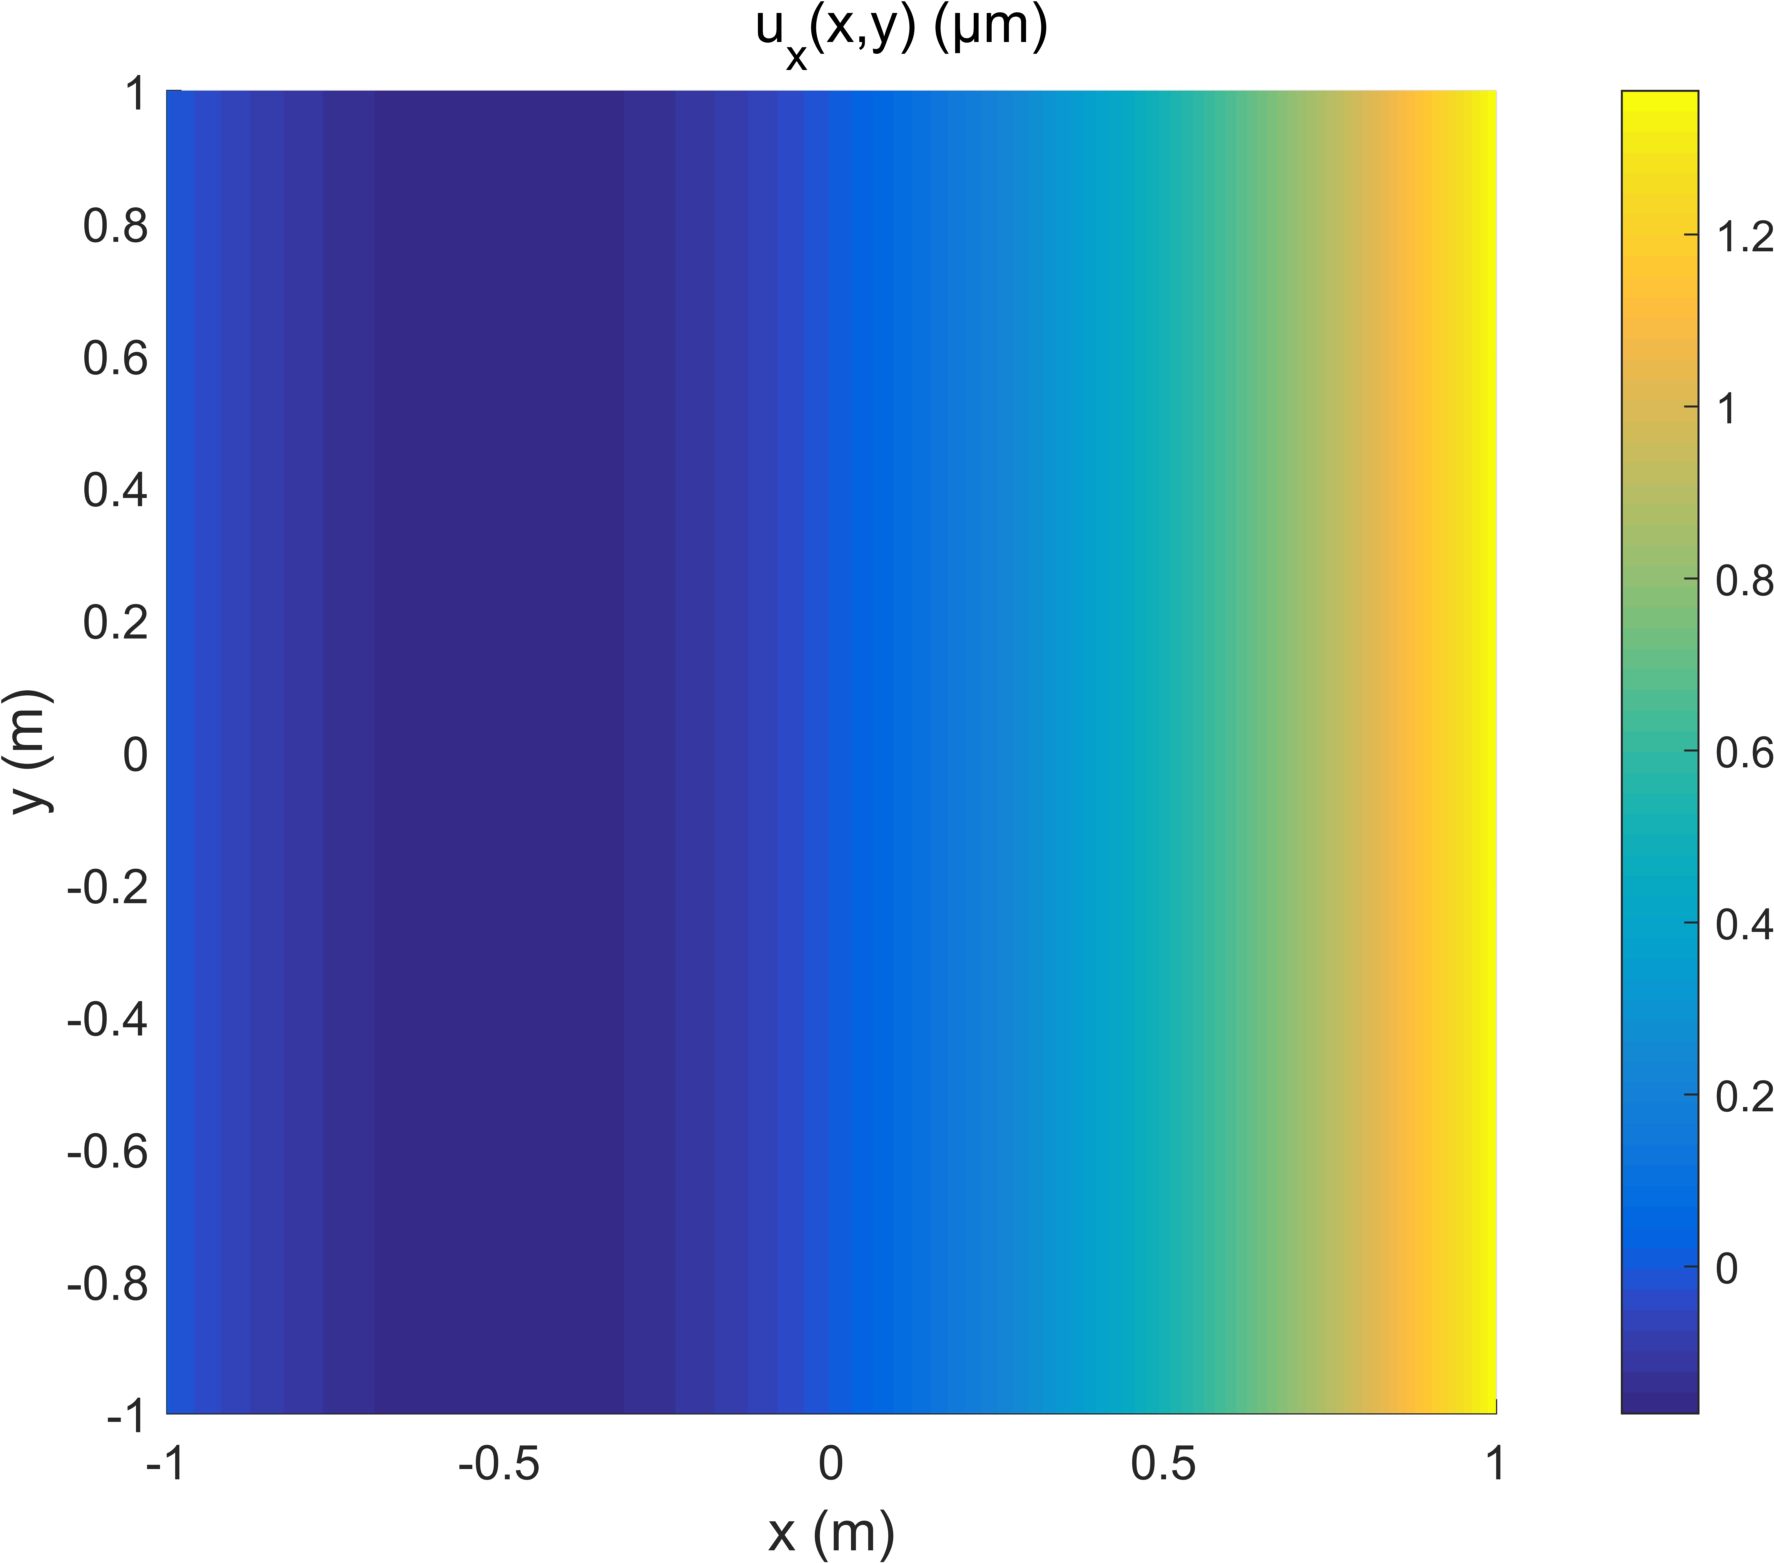
\includegraphics[width=\linewidth]{q2a_surf_ux.png}
	\end{subfigure}%
	\begin{subfigure}{.5\textwidth}
		\centering
		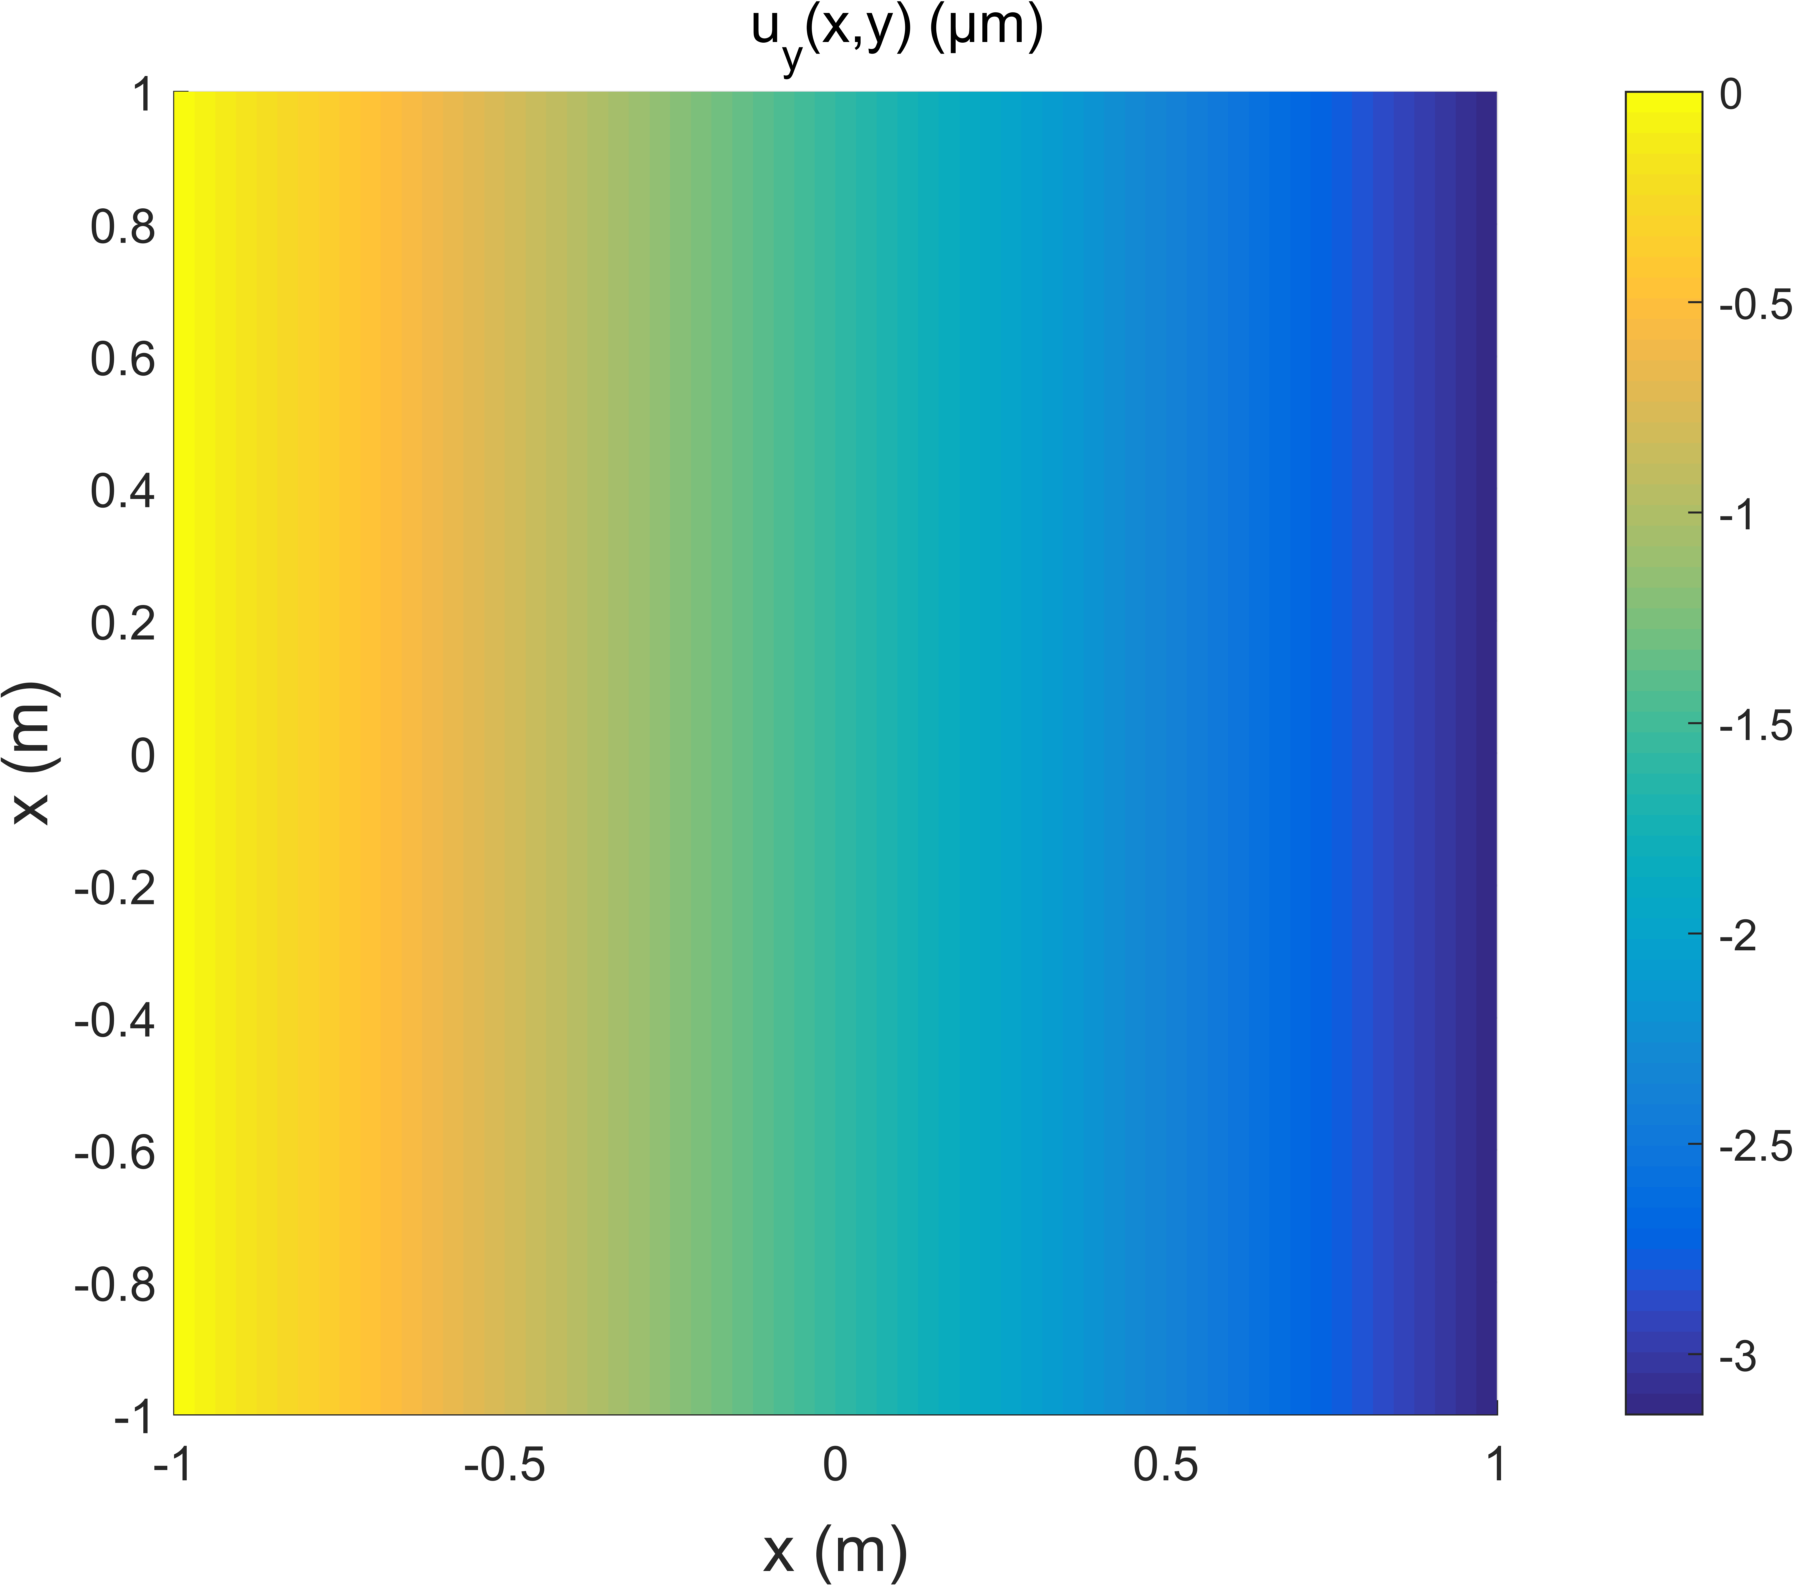
\includegraphics[width=\linewidth]{q2a_surf_uy.png}
	\end{subfigure}
	\caption{Deflection of the single square element beam in the $x$-direction, $u_x(x,y)$ (in units of \SI{}{\micro\m}) is shown on the left with deflection in the $y$-direction, $u_y(x,y)$ (in units of \SI{}{\micro\m}) on the right.}
	\label{fig:q2a_ux_uy}
\end{figure}

\begin{figure}[h!]
	\centering
	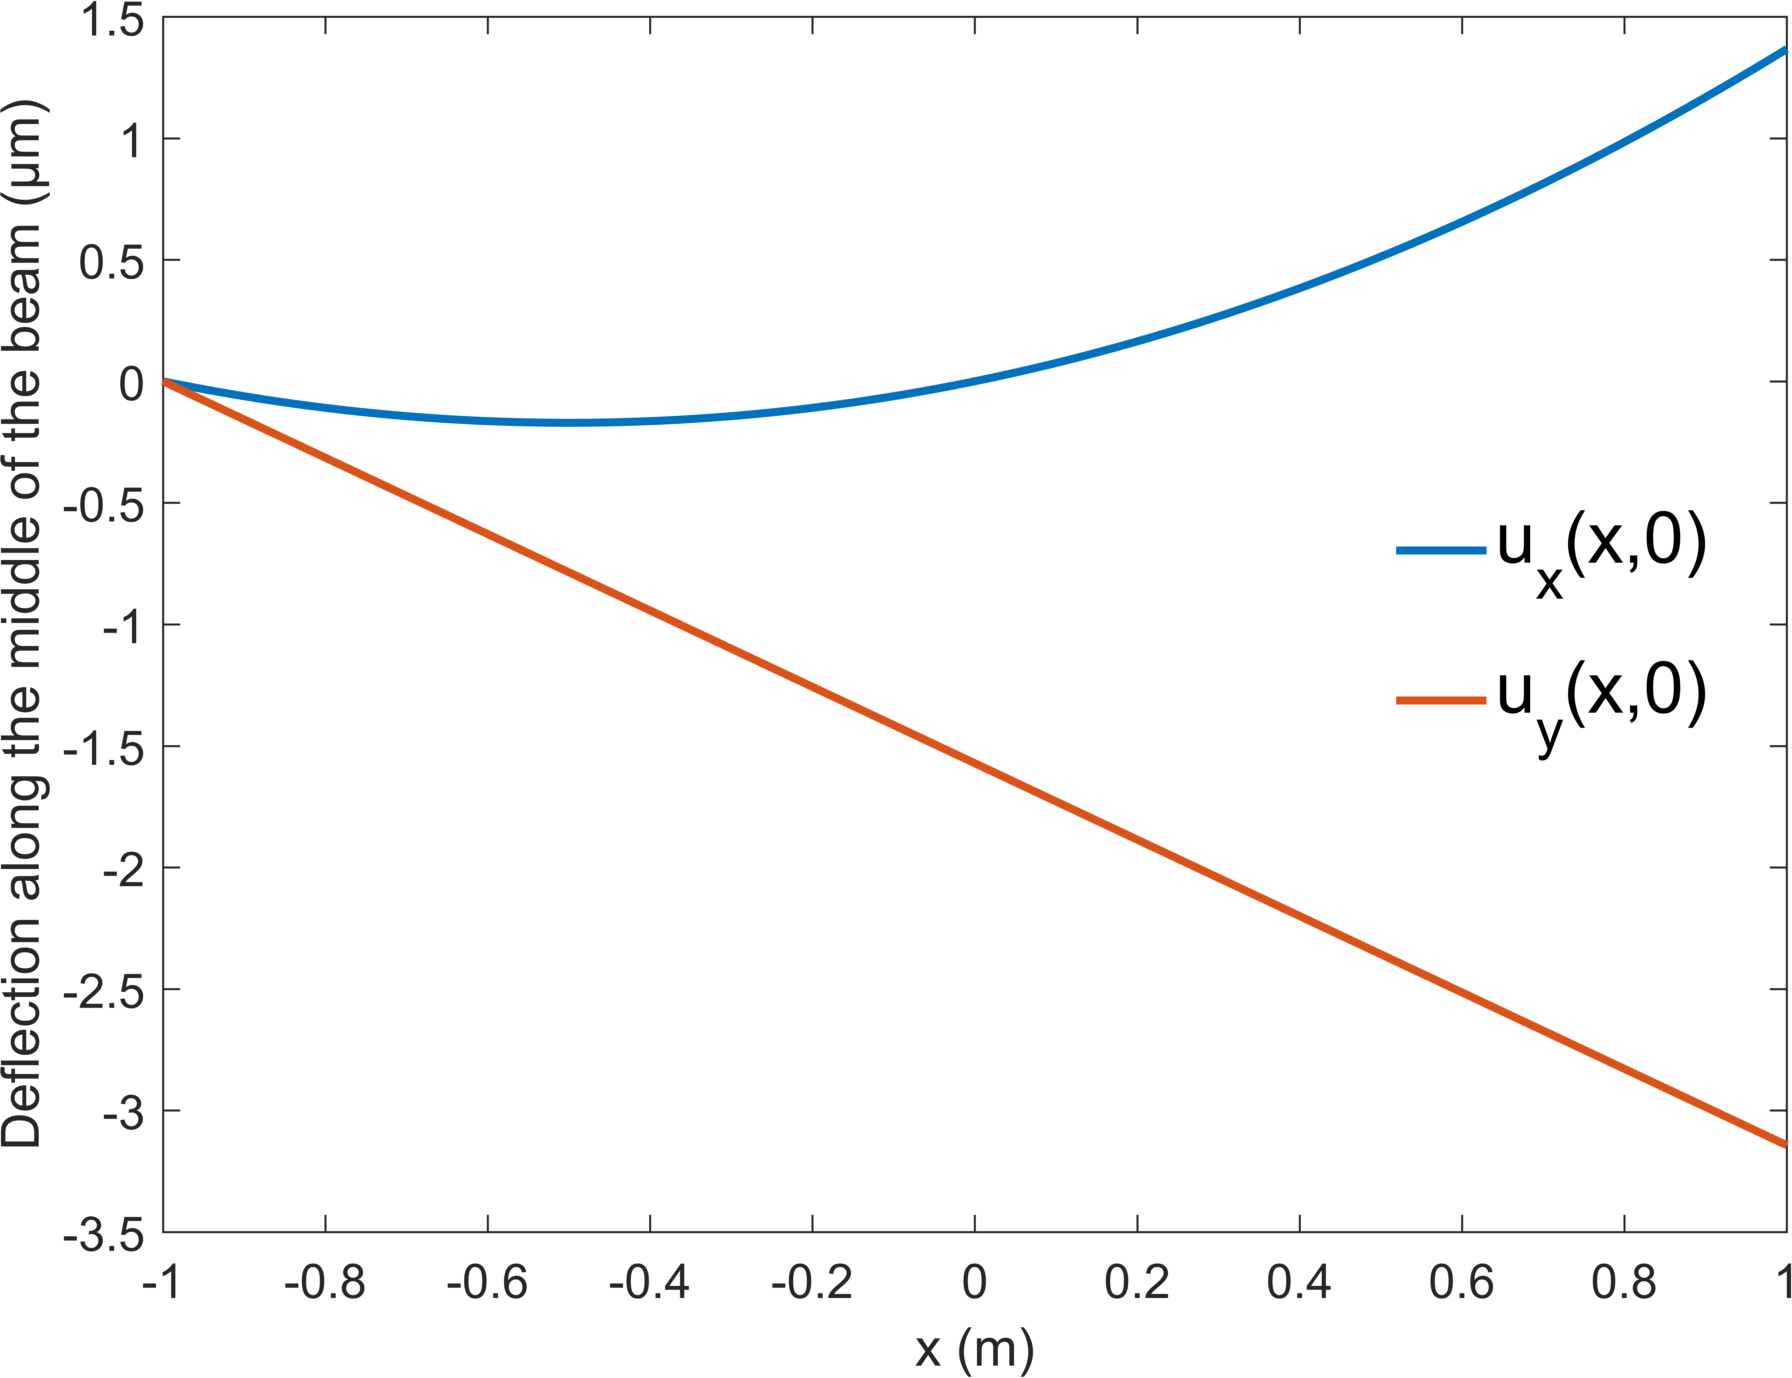
\includegraphics[width=0.7\linewidth]{q2a_plot.png}
	\caption{Deflection of the single square element beam along the middle of the beam ($y=0$) in the $x$-direction, $u_x(x,0)$ and the deflection along the middle of the beam in the $y$-direction, $u_y(x,0)$.}
	\label{fig:q2a_plot}
\end{figure}

\begin{thebibliography}{9}
\bibitem{Tchonkova011}
Tchonkova, M. and Sture, S., (2001). Classical and recent formulations for linear elasticity. \textit{Archives of Computational Methods in Engineering} \textbf{8}(1), pp. 41--74.

\bibitem{mathworld}
Rowland, T. Symmetric Bilinear Form. From MathWorld--A Wolfram Web Resource, created by Eric W. Weisstein. \url{http://mathworld.wolfram.com/SymmetricBilinearForm.html}

\bibitem{Mott09}
Mott, P. H., and C. M. Roland, (2009). Limits to Poisson's ratio in isotropic materials. \textit{Physical Review B} \textbf{80}(13), 132104.
\end{thebibliography}

\end{document}